\documentclass{article}

\usepackage{fancyhdr}
\usepackage{extramarks}
\usepackage{amsmath}
\usepackage{amssymb}
\usepackage{amsthm}
\usepackage{amsfonts}
\usepackage{graphicx,wrapfig}
\usepackage{booktabs}

\usepackage{caption}
\usepackage{subcaption}
\usepackage{tikz}
\usetikzlibrary{automata,positioning}

\usepackage[plain]{algorithm}
\usepackage{algpseudocode}

\usepackage{hyperref}
\hypersetup{
    colorlinks,
    citecolor=black,
    filecolor=black,
    linkcolor=black,
    urlcolor=black
}



%
% Basic Document Settings
%

\topmargin=-0.45in
\evensidemargin=0in
\oddsidemargin=0in
\textwidth=6.5in
\textheight=9.0in
\headsep=0.35in

\linespread{1.1}

\pagestyle{fancy}
\lhead{\hmwkAuthorName}
\chead{\hmwkClass\ (\hmwkClassInstructor)}
\rhead{\hmwkTitle}
% \lfoot{\lastxmark}
\cfoot{\thepage}

\renewcommand\headrulewidth{0.4pt}
\renewcommand\footrulewidth{0.4pt}

\setlength\parindent{0pt}

%
% Details
%   - Title
%   - Due date
%   - Class
%   - Section/Time
%   - Instructor
%   - Author
%

\newcommand{\hmwkTitle}{ARMv7 Architecture}
\newcommand{\hmwkDueDate}{March 7th, 2018}
\newcommand{\hmwkClass}{MC}
% \newcommand{\hmwkClassTime}{}
\newcommand{\hmwkClassInstructor}{Dr. Suma M N}
\newcommand{\hmwkAuthorName}{Akshit Bhalla}


\renewcommand{\part}[1]{\textbf{\large Part \Alph{partCounter}}\stepcounter{partCounter}\\}

%
% Various Helper Commands
%

% Useful for algorithms
\newcommand{\alg}[1]{\textsc{\bfseries \footnotesize #1}}

% For derivatives
\newcommand{\deriv}[1]{\frac{\mathrm{d}}{\mathrm{d}x} (#1)}

% For partial derivatives
\newcommand{\pderiv}[2]{\frac{\partial}{\partial #1} (#2)}

% Integral dx
\newcommand{\dx}{\mathrm{d}x}

% Alias for the Solution section header
\newcommand{\solution}{\textbf{\large Solution}}

% Probability commands: Expectation, Variance, Covariance, Bias
\newcommand{\E}{\mathrm{E}}
\newcommand{\Var}{\mathrm{Var}}
\newcommand{\Cov}{\mathrm{Cov}}
\newcommand{\Bias}{\mathrm{Bias}}

\begin{document}

\title{\fontsize{14pt}{16.8pt}\selectfont\bf{SELF STUDY}}
\date{}

\maketitle
\thispagestyle{empty}

\begin{center}
\vspace*{-15mm}

{\fontsize{14pt}{16.8pt}\selectfont\textit{in}} \\
\vspace*{5mm}

{\fontsize{14pt}{16.8pt}\selectfont\textbf{MICROCONTROLLERS [15ES4GCMCS]}} \\

\vspace*{5mm}
{\fontsize{14pt}{16.8pt}\selectfont\textbf{ARMv7 Architecture}}

\vspace*{5mm}
{\fontsize{14pt}{16.8pt}\selectfont\textit{by}} \\
\vspace*{6mm}

\author{\fontsize{14pt}{16.8pt}\selectfont\textbf{Akshit Bhalla}}\\
\vspace*{2mm}
{\fontsize{12pt}{14.4pt}\selectfont\textit{[1BM16EC015]} } \\



\vspace*{3mm}

\vspace*{4mm}\fontsize{14pt}{16.8pt}\selectfont\textit{Under the supervision of} \\
\vspace*{2mm}\fontsize{14pt}{16.8pt}\selectfont\textbf{Dr. Suma M N} \\
\vspace*{8mm}

\begin{figure}[H]
\centering
  
\includegraphics[height=36mm,width=36mm]{assets/BMSCE_Logo.png}
\end{figure}

\vspace*{3mm}

{\fontsize{14pt}{16.8pt}\selectfont\textbf{March 7th, 2018}} \\

\vspace*{5mm}

\fontsize{14pt}{16.8pt}\selectfont\textbf{Department of Electronics and Communication Engineering \\
\vspace*{4mm}
\vspace*{2mm} B.M.S COLLEGE OF ENGINEERING, Basavanagudi} \\
\vspace*{2mm}
\fontsize{14pt}{16.8pt}\selectfont\textbf{Bangalore-560019, India} 
\vspace*{10mm}\\

\end{center}
 % cover page
\thispagestyle{empty}
\newpage

% \maketitle

\graphicspath{{assets/}} % path to images folder

\pagebreak

\newpage

\setcounter{page}{1} 


\section{Introduction}\label{section:intro}

The hardware board chosen for this project is the Pico i.MX7D, which implements the ARM Cortex-A7 core, which operates at speeds of up to 1.2 GHz, as well as the ARM Cortex-M4 core. The dual-core
architecture enables the device to run a rich operating system like Linux on the Cortex-A7 core and an RTOS
on the Cortex-M4 core.\\
\newline
The ARM Cortex-M4 and Cortex-A7 range of microcontroller cores are high performance and
low power 32-bit RISC processors.

\begin{figure}[H]
  \makebox[\textwidth][c]{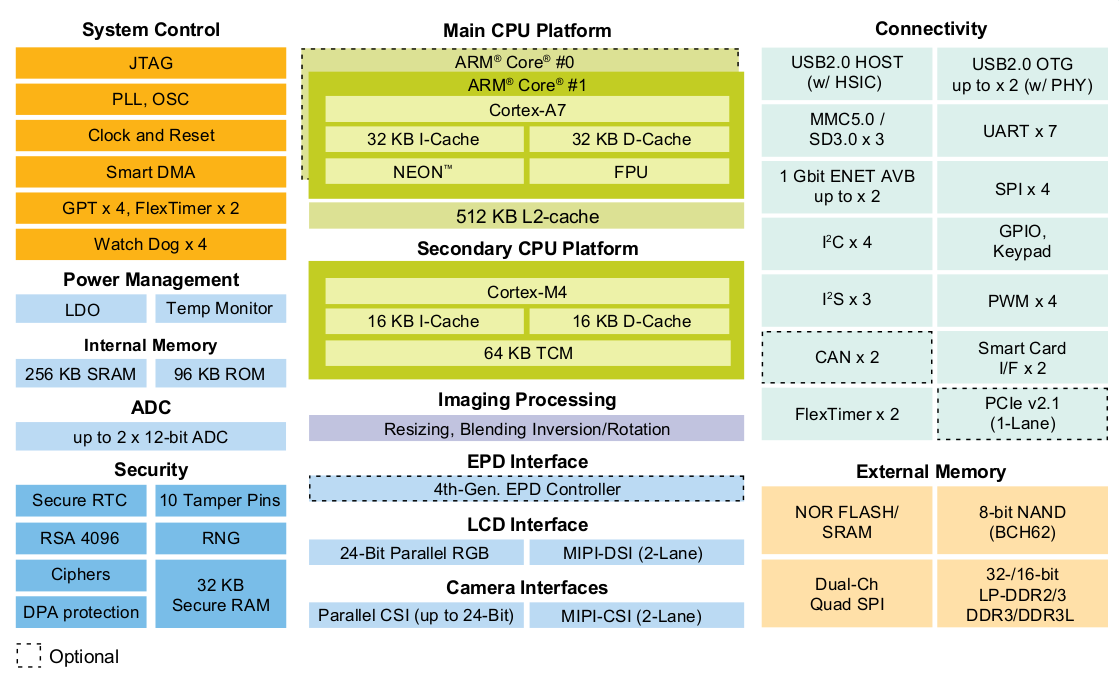
\includegraphics[width=1.1\textwidth]{block-diag}}%
  \caption{ Block Diagram of Pico i.MX7D}
  \label{block-diag}
\end{figure}

\subsection{Cortex-A7} \label{subsection:Cortex-A7}

The Application-A profile defines an architecture aimed at high performance
processors, supporting a virtual memory system using a Memory Management
Unit (MMU) and therefore capable of running fully featured operating systems.
Support for the ARM and Thumb instruction sets is provided

\begin{itemize}
    \item Modified Harvard Architecture (separate, concurrent access to instructions and data).
    \item Load/Store Architecture.
    \item Thumb-2 technology as standard. \((discussed\; under\; Cortex-M4)\)
    \item Less than \(0.5mm^2\), using \(28nm\) process technology.
    \item Floating Point Unit (FPU)
  \end{itemize}

\newpage
\subsection{Cortex-M4} \label{subsection:Cortex-M4}

The Microcontroller-M profile defines an architecture aimed at low cost systems,
where low-latency interrupt processing is vital. Cortex-M processors differ from other processors in
ARM’s range in that they execute only Thumb-2 instructions and do not support the complete ARM
instruction set.
\begin{wrapfigure}{r}{0.17\textwidth}
    \begin{center}
      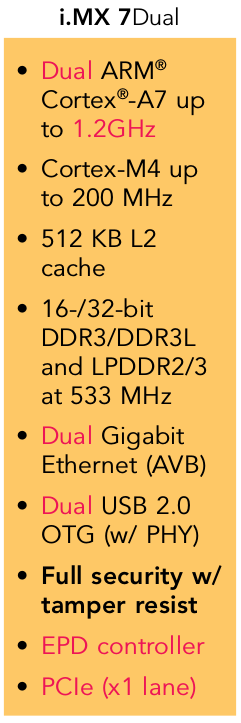
\includegraphics[width=0.19\textwidth]{features}
    \end{center}
    \caption{Features}
\end{wrapfigure}

\begin{itemize}
    \item Efficient Harvard architecture 3-stage pipeline core (Fetch-Decode-Execute). 
    \item 32-bit processor, including 32-bit address and data buses.
    \item 4GB address space and up to 2GB for RAM (either on or off chip).
    \item A Nested Vectored Interrupt Controller (NVIC) for low-latency interrupt processing.
    \item Memory Protection Unit (MPU).
    \item Fixed Memory Map for easy porting of software between systems based on Cortex-M4.
  \end{itemize}

\vspace*{2mm}

\subsection*{Thumb Instruction Set} \label{subsection:Thumb}

Thumb instructions are each 16 bits long, and have a corresponding 32-bit ARM instruction that has the same effect. The main reason for using Thumb code is to reduce code density. Because of its
improved density, Thumb code tends to cache better than the equivalent ARM code and can
reduce the amount of memory required. The complete ARM instruction set may be used for particular code sections which require the highest performance.\\

\subsection{I/O} \label{subsection:I/O}

\begin{enumerate}
    \item Communication Ports (I2C, SAI, UART, SPI, SDIO, USB, PCIe).
    \item Parallel and MIPI CSI Camera Interfaces.
    \item Parallel RGB and MIPI DSI Display Interfaces. The processor integrates an EPD controller that supports E-INK color and monochrome panels with up to 2048 x 1536 resolution at 106 Hz refresh, 4096 x 4096 resolution at 20 Hz refresh and 5-bit grayscale (32-levels per color channel).
    \item 2 x 10/100/1000 Mbps Ethernet controllers.
    \item The multilevel Cortex-A7 memory system is based on the L1 instruction and data caches, L2 cache, and internal and external memory. The processor supports many types of external memory devices, including DDR3, DDR3L, LPDDR2 and LPDDR3, NOR Flash, NAND Flash (MLC and SLC), QSPI Flash.
  \end{enumerate}

\newpage

\section{Comparision with 8051}\label{section:8051}

Direct comparisons between two such different products are difficult.
Both are available in many different configurations. The Cortex-M series is arguably more standardized than the 8051, which exists in several different variants (some of which are obsolete).\\
\newline
For the purposes of comparison, I've selected two devices from chip manufacturer
Atmel. For the 8051 architecture, we will look at the AT89C51RD2; for the ARMv7-M, the
SAM3S1A (Cortex-M3).\\
\newline

\begin{figure}[H]
    \makebox[\textwidth][c]{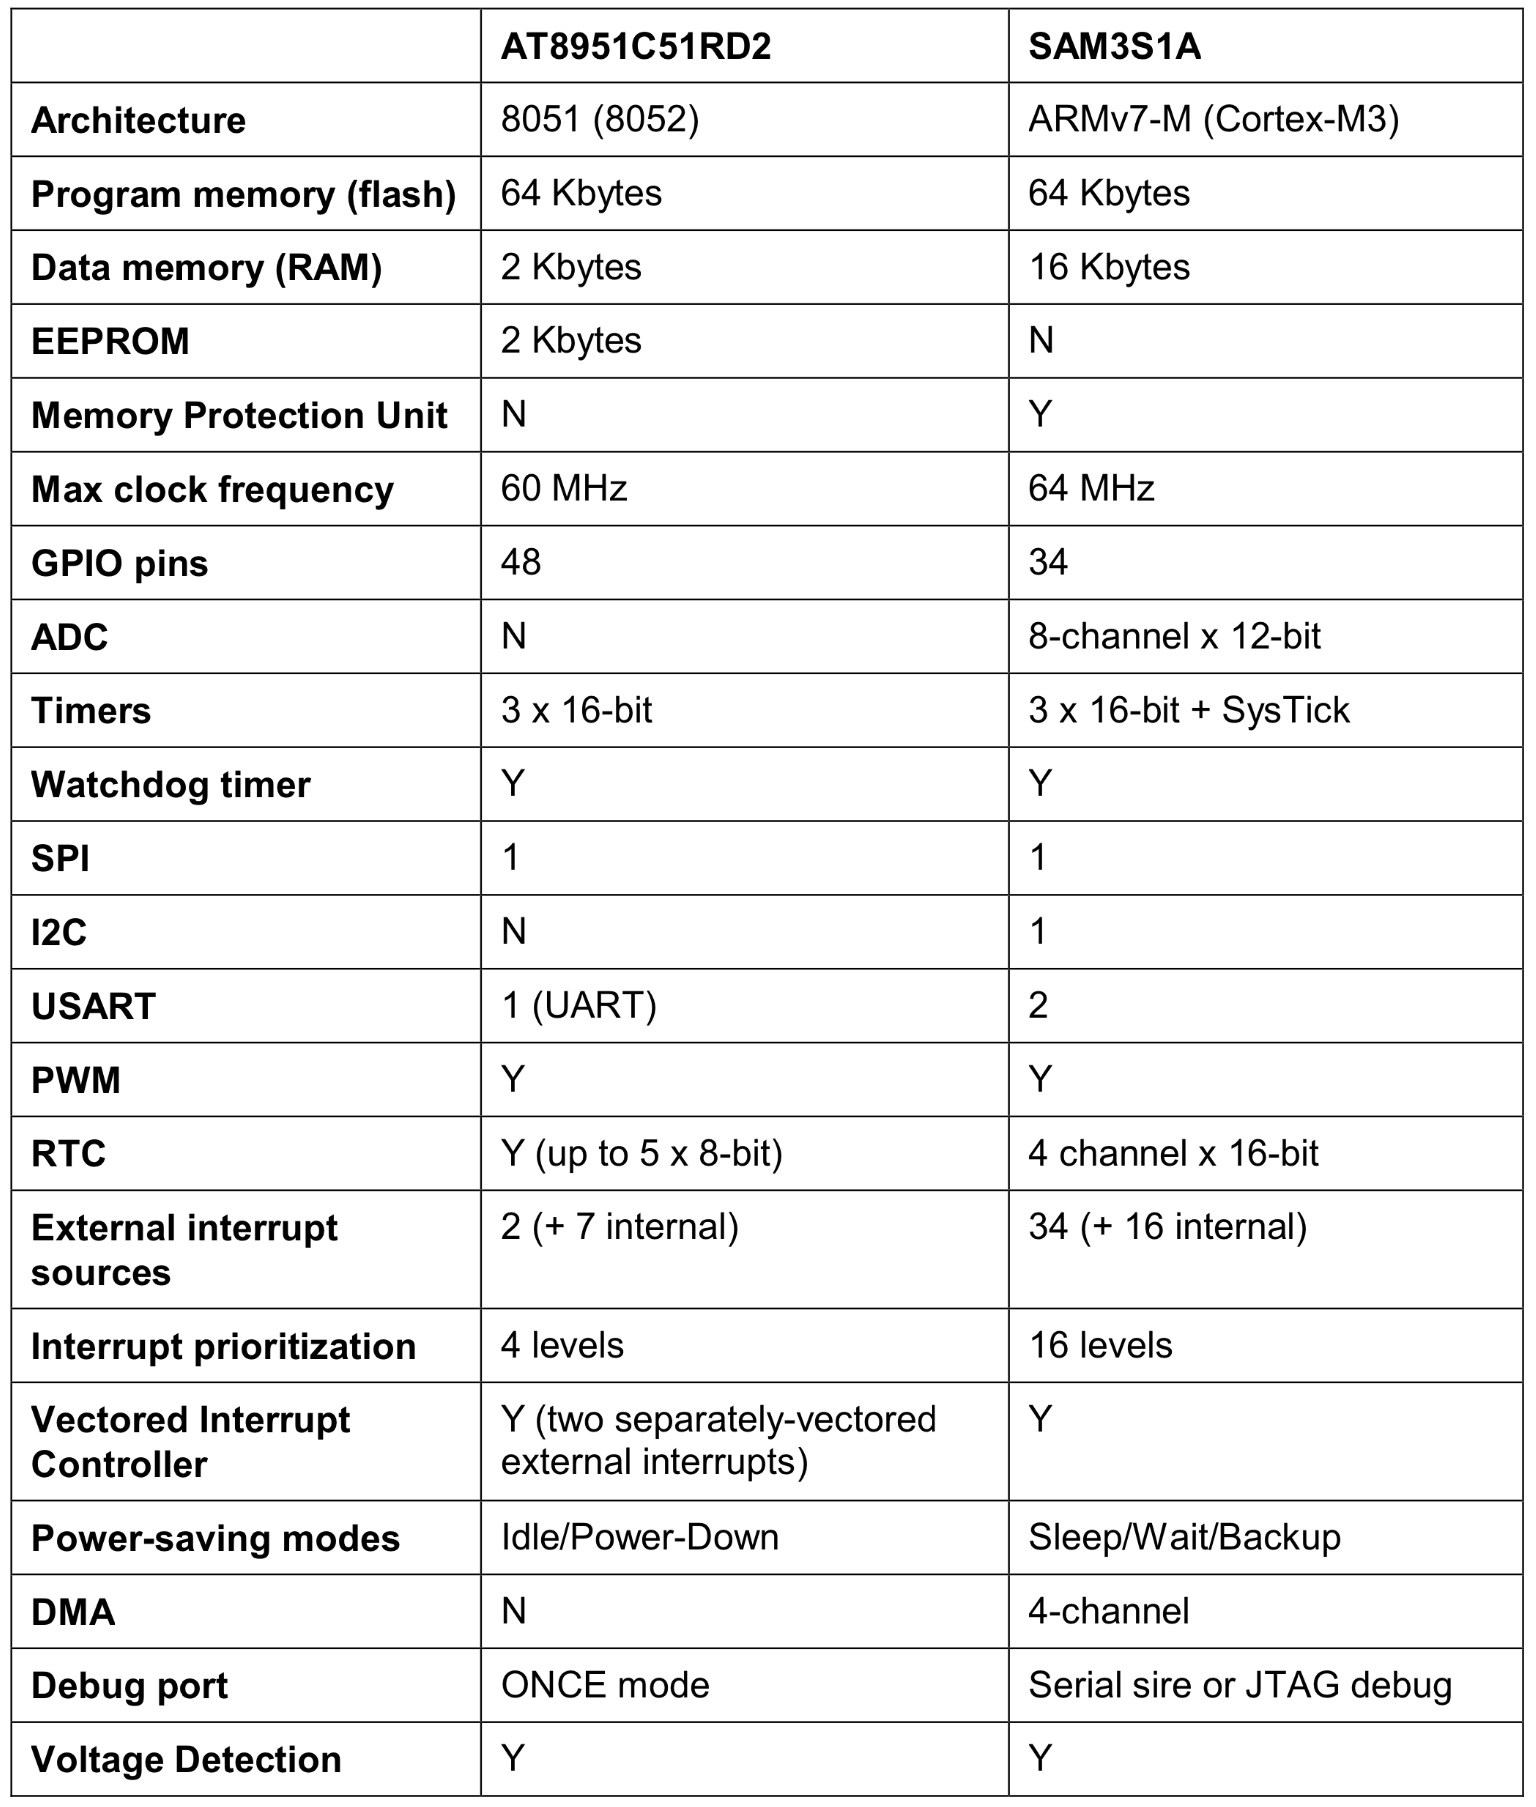
\includegraphics[scale=0.27]{8051}}%
    \caption{ Comparision Table }
    \label{8051}
  \end{figure}
  
\newpage
  \subsection{Register Set} \label{subsection:Registers} 

  \begin{enumerate}
    \item 8051:
    \begin{enumerate}
      \item Two 8-bit registers (ACC and B) which are generally used in arithmetic and logic instructions.
      \item 16-bit address register, DPTR, which is used
      exclusively for addressing external memory.
      \item 4 banks of eight 8-bit registers which are mapped into the first 32 bytes
      of internal RAM. These are byte and bit addressable. The bank in current use is selected
      via the RS0 and RS1 bits in the PSW (see below).
      \end{enumerate}
    \item ARMv7-M
    \begin{enumerate}
            \item 16 32-bit registers, R0-R15. R0-R12 are generally available for
            essentially all instructions.
            \item R13 is used as the Stack Pointer, R14 as the Link Register (for
            subroutine and exception return) and R15 as the Program Counter. None of the registers are directly addressable.
            \item Since the registers are all 32-bit, it supports 32-bit arithmetic and logic
            operations efficiently.
    \end{enumerate}
  \end{enumerate}

  \subsection{Addressing Modes} \label{subsection:Addressing Modes}

\vspace*{2mm}
\begin{table}[H]
  \centering
  \begin{tabular}{@{}|l|l|l|@{}}
  \toprule
  \textbf{Name}                                                                 & \textbf{Alternative Name}              & \multicolumn{1}{c|}{\textbf{ARM Examples}}                              \\ \midrule
  Register to Register                                                          & Register Direct                        & MOV R0, R1                                                              \\ \midrule
  Absolute                                                                      & Direct                                 & LDR R0, MEM                                                             \\ \midrule
  Literal                                                                       & Immediate                              & \begin{tabular}[c]{@{}l@{}}MOV R0, \#15\\ ADD R1, R2, \#12\end{tabular} \\ \midrule
  Indexed, Base                                                                 & Register Indirect                      & LDR R0, {[}R1{]}                                                        \\ \midrule
  \begin{tabular}[c]{@{}l@{}}Pre-Indexed,\\ Base with Displacement\end{tabular} & Register Indirect with Offset          & LDR R0, {[}R1, \#4{]}                                                   \\ \midrule
  Pre-Indexed                                                                   & Register Indirect Pre-Increment        & LDR R0, {[}R1, \#4{]}!                                                  \\ \midrule
  Post-Indexed                                                                  & Register Indirect Post-Increment       & LDR R0, {[}R1{]}, \#4                                                   \\ \midrule
  Double Register Indirect                                                      & Register Indirect Register-Indexed     & LDR R0, {[}R1, R2{]}                                                    \\ \midrule
  Double Register Indirect with Scaling                                         & Register Indirect Indexed-with-Scaling & LDR R0, {[}R1, r2, LSL \#2{]}                                           \\ \midrule
  Program Counter Relative                                                      &                                        & LDR R0, {[}PC, \#offset{]}                                              \\ \bottomrule
  \end{tabular}
  \caption{Types of Addressing Modes}
  \label{Addressing Modes}
  
  \vspace*{2mm}
  \begin{enumerate}
    \item For Thumb Instructions, the destination register cannot be PC (Program Counter) or SP (Stack Pointer).
    \item For ARM instructions:
    \begin{enumerate}
      \item Destination must be an even-numbered register.
      \item Destination must not be LR (Link Register).
      \item In a double-word (64-bit) destination, second destination register must be R(t + 1).
    \end{enumerate}
  \end{enumerate}

  \end{table}  \subsection{Status Registers} \label{subsection:Status Registers} 

  \begin{itemize}
      \item The 8051 PSW register contains Carry (CY), Auxiliary Carry (AC) and Overflow (OV) flags
      (set on results from ALU operations), RS0 and RS1 (used to select one of four register
      banks in current use) and a parity flag, P (set by the hardware to indicate whether there
      are an even or odd number of set bits in the accumulator on each instruction cycle).
      \item The Cortex-M4 Program Status Register (xPSR) is a single 32-bit register with several
      aliases, each providing a view of a different subset of the contents.\\ From the user point of
      view, the Application Program Status Register (APSR) contains the ALU status flags. For
      operating system and exception handling use, the Interrupt Program Status Register
      (IPSR) contains the number of the currently executing interrupt (or zero if none are currently
      active). The Execution Program Status Register (EPSR) contains bits which reflect
      execution status and is not directly accessible.
  \end{itemize}
  
  \begin{figure}[H]
    \makebox[\textwidth][c]{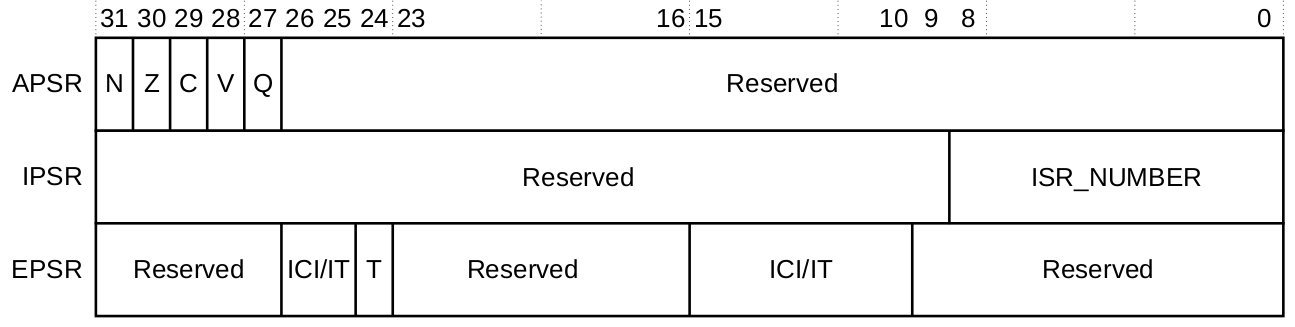
\includegraphics[width=1.1\textwidth]{PSR}}%
    \caption{The Program Status Register (xPSR) combines APSR, IPSR and EPSR}
    \label{PSR}
  \end{figure}

\subsection{Stack}\label{subsection:Stack}

\begin{enumerate}
  \item 8051:
  \begin{enumerate}
    \item The 8051 supports a Full Ascending stack (byte-sized) using a single stack pointer, SP. 
    \item SP is initialized to 0x07, meaning that the first item pushed on to the stack goes to address 0x08.
    \item It cannot grow beyond the end of internal RAM at 0xFF. This means that the 8051 only supports 248 bytes of stack space.
    \item The 8051 stack pointer is typically initialized to the address one byte below the start of the
    allocated stack area so that the first push uses the first byte of the area (since the stack
    model is Full Ascending the stack pointer is incremented before the first store).
    \end{enumerate}
  \item ARMv7-M
  \begin{enumerate}
          \item The Cortex-M4 supports a Full Descending stack (word-sized, 32 bits) addressed by the current stack pointer.
          \item This stack can be located anywhere in RAM. Typically, for best performance,
          it will be located in internal SRAM. Stack size is limited only by the available RAM space.
          \item The stack pointer is typically initialized to the word above the top of the
          allocated stack area. Since the stack model is Full Descending, the stack pointer is
          decremented before the first store, thus placing the first word on the stack at the top of the
          allocated region.
  \end{enumerate}
\end{enumerate}

\section{Programming}\label{section:Programming}

The 8051 architecture strictly segregates code and data within the memory map. Further,
it requires that data items be assigned to one of the available memory regions.
\begin{itemize}
  \item \textbf{data} Internal on-chip RAM, directly addressed using 8-bit addresses and
  restricted to 128 bytes or less.
  \item \textbf{idata} Internal on-chip RAM, indirectly accessed using 8-bit addressing. Limited
  to 256 bytes, the lower half of which overlaps the data region.
  \item \textbf{bdata} Internal on-chip bit-addressable RAM.
  \item \textbf{xdata} External data memory, accessed using 16-bit addressing and restricted to
  64Kbytes or less.
  \item \textbf{pdata} One page of external data memory, limited to 256 bytes and accessed
  using 8-bit addressing.
\end{itemize}


The ARMv7-M architecture of the Cortex-M4 supports a single, unified address space. All
memory access instructions can be used to address items in all regions of memory. This
is much more flexible, allowing code and data to be essentially freely allocated across all
available memory regions. 

\begin{figure}[H]
  \makebox[\textwidth][c]{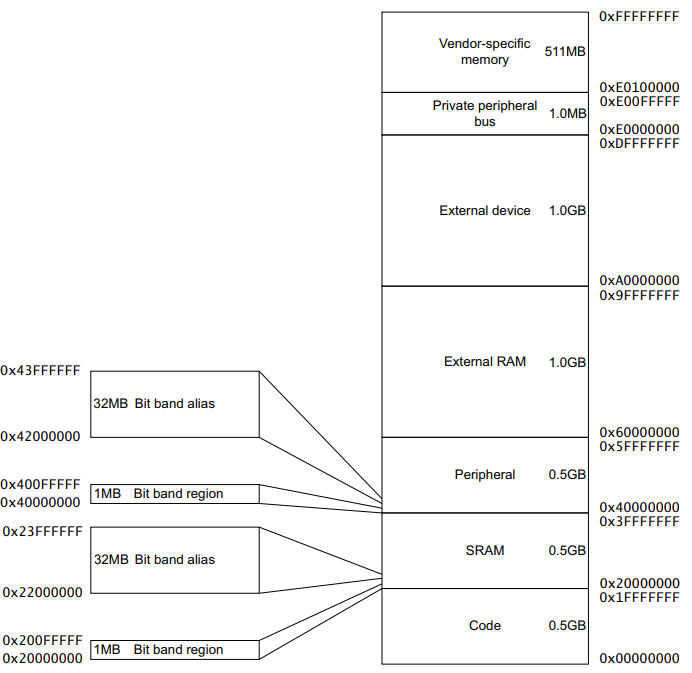
\includegraphics[width=0.8\textwidth]{memory}}%
  \caption{Cortex-M4 Memory Map}
  \label{block-diag}
\end{figure}

\subsection{Data Types}\label{subsection:DataTypes}

The ARMv7-M is a 32-bit architecture and, as such, handles 32-bit types very efficiently.
In particular, 8-bit and 16-bit types are less efficiently manipulated, although they will save
on data memory if this is an issue.\\
\newline
The sbit keyword is used to declare items which are bit-addressable on 8051. This is
unnecessary in the Cortex-M4 as bit-banding provides bit-addressable accesses via
standard memory access instructions to aliased addresses.

\begin{figure}[H]
  \makebox[\textwidth][c]{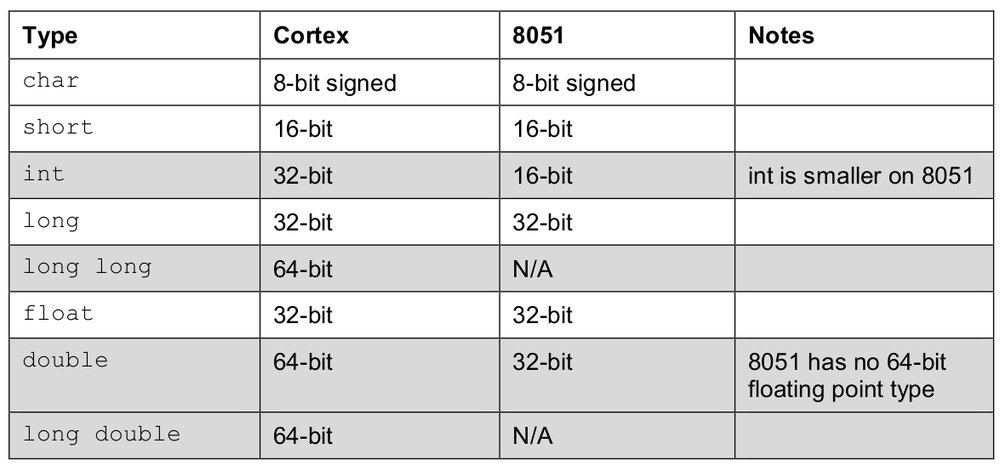
\includegraphics[width=0.75\textwidth]{data-types}}%
  \caption{Data Types}
  \label{data-types}
\end{figure}

\subsection{IDE Availability}\label{subsection:IDE}

There are numerous software options avaialable for development on the ARMv7 platform. Some of the popular IDEs are listed below.

\begin{itemize}
  \item Keil MDK - ARM
  \item Visual Studio by Microsoft as IDE, with GNU Tools as compiler/linker
  \item GNU ARM Eclipse
  \item ARM Development Studio 5
  \item Atmel Studio (for Atmel manafactured microcontrollers)
\end{itemize}

\(Important:\) Cortex-A7 and Cortex-M4 are immune to the recently discovered Spectre and Meltdown vulnerabilities found in Intel x86, AMD and various other chips due to the nature in which Speculation Processing is handled in these cores.
\\\texttt{https://www.raspberrypi.org/blog/why-raspberry-pi-isnt-vulnerable-to-spectre-or-meltdown/}

\begin{verbatim}
Sample Code: 
  
  1. @ Hello World
      .global _start
      _start:
        MOV R7, #4 @ Syscall to output to screen
        MOV R0,  #1 @ Monitor output stream
        MOV R2, #12 @ String Length
        LDR R1, =message @ Load register with address of string
        SWI 0
      end:
        MOV R7, #1 @ Exit syscall
        SWI 0
      .data @ Signify that what follows is data
      message:
        .ascii "Hello World\n"
    
  2. Multiply values (Must store values in Registers)

      .global _start
      _start:
      MOV R1, #0x14 @ Put 20 in R1
      MOV R2, #0xA @ Put 10 in R2
      MUL R0, R1, #0xA @ Multiply 20 * 10, store in R0
      MOV R7, #1 @ Exit with a system call
      SWI 0 @ End program and return to terminal

  3. Compare 2 Values

    .global _start
      _start:
        MOV R1, #5
        MOV R2, #10
        CMP R1, R2 @ Compare values setting flags
        BEQ vals_equal @ If equal jump to vals_equal (Zero Flag Set)
        BGT r1_gt @ If R1 is greater jump to r1_gt (Negative Flag Set)
      @ Come here next by default
      r1_lt:
        MOV R0, #2
        B end
      r1_gt:
        MOV R0, #3
        B end
      vals_equal:
        MOV R0, #1
      end:
        MOV R7, #1 
        SWI 0
\end{verbatim}

\begin{thebibliography}{9}
  \bibitem{Cortex-M4} 
  
  \textit{Cortex-M4 Technical Reference Manual}. 
  ARM, 1993.
  \\\texttt{https://developer.arm.com/docs/100166/0001}
   
  \bibitem{Pico} 
  Pico i.MX7D 
  \textit{Datasheet}. 
  NXP, 2017.
  \\\texttt{https://www.nxp.com/docs/en/data-sheet/IMX7DCEC.pdf}
  \end{thebibliography}

\end{document}
